\documentclass[11pt,a4paper]{report}

% Aberstwyth dissertation LaTeX Template
% Authors: Dr. Hannah Dee (hmd1@aber.ac.uk), Neil Taylor (nst@aber.ac.uk)
% This has been adapted from the Leeds Thesis template and the 
% Group Project template for Computer Science in Aberystywth University.
% 
% All comments and suggestions welcome.
%
% Template designed to be used with pdflatex: it may need alteration to
% run with a different LaTeX engine

% To build document on the unix command line, run four commands:
 
% pdflatex dissertation
% bibtex dissertation
% pdflatex dissertation
% pdflatex dissertation

% you will end up with dissertation.pdf 
\usepackage{mmp}

% the following packages are used for citations - You only need to include one. 
%
% Use the cite package if you are using the numeric style (e.g. IEEEannot). 
% Use the natbib package if you are using the author-date style (e.g. authordate2annot). 
% Only use one of these and comment out the other one. 
\usepackage{cite}
%\usepackage{natbib}

% Use the following to selectively exclude chapters
%\includeonly{cover,abstract,acknowledge,declare,chapter1,chapter2}

\begin{document}

% all of the include directives below refer to tex files
% so 
\title{A Toolkit For Reporting On Metagenome Assembly Quality}

% Your name
\author{James Edward Euesden}

% Your email 
\authoremail{jee22@aber.ac.uk}

\degreeschemecode{G401} %e.g. G400 
\degreeschemetitle{Computer Science} % e.g. Computer Science
\degreetype{BSc}

\modulecode{CS39440} % i.e. CS39440, CC39440, CS39620
\moduletitle{Major Project} % i.e. Major Project or Minor Project

\date{1st May 2016} % i.e. the date of this version of the report

\status{Release} % Use draft until you create the release version. Then, change this to Release.
\version{1.0}

%The title and name of your supervisor.
\supervisor{Amanda Clare} 

%The email for your supervisor. 
\supervisoremail{afc@aber.ac.uk}

\maketitle



 includes cover.tex - to change the content,
% edit the tex file

\pagenumbering{roman}

% This is the front page

\title{A Toolkit For Reporting On Metagenome Assembly Quality}

% Your name
\author{James Edward Euesden}

% Your email 
\authoremail{jee22@aber.ac.uk}

\degreeschemecode{G401} %e.g. G400 
\degreeschemetitle{Computer Science} % e.g. Computer Science
\degreetype{BSc}

\modulecode{CS39440} % i.e. CS39440, CC39440, CS39620
\moduletitle{Major Project} % i.e. Major Project or Minor Project

\date{1st May 2016} % i.e. the date of this version of the report

\status{Release} % Use draft until you create the release version. Then, change this to Release.
\version{1.0}

%The title and name of your supervisor.
\supervisor{Amanda Clare} 

%The email for your supervisor. 
\supervisoremail{afc@aber.ac.uk}

\maketitle



                        

% Set up page numbering
\pagestyle{empty}

% declarations of originality 
\thispagestyle{empty}

%%%
%%% You must sign the declaration of originality. 
%%%
\begin{center}
    {\LARGE\bf Declaration of originality}
\end{center}

In signing below, I confirm that:

\begin{itemize}
\item{This submission is my own work, except where 
clearly indicated.}

\item{I understand that there are severe penalties for 
Unacceptable Academic Practice, which can lead to loss 
of marks or even the withholding of a degree.}
 
\item{I have read the regulations on Unacceptable Academic 
Practice from the University's Academic Quality and 
Records Office (AQRO) and the relevant sections of the 
current Student Handbook of the Department of 
Computer Science.}
 
\item{In submitting this work I understand and agree to 
abide by the University's regulations governing these issues.}
\end{itemize}

\vspace{2em}
Name ............................................................  \\

\vspace{1em}
Date ............................................................ \\

%%% 
%%% We would like to make a selection of final reports available to students that take 
%%% this module in future years. To enable us to do this, we require your consent. You 
%%% are not required that you do this, but if you do give your consent, then we will have 
%%% the option to select yours as one of a number of reports as examples for other 
%%% students. If you would like to give your consent, then please include the following 
%%% text and sign below. If you do not wish to give your consent, please remove this 
%%% from your report. 
%%%
\vspace{1em}
\begin{center}
    {\LARGE\bf Consent to share this work}
\end{center}

In signing below, I hereby agree to this dissertation being made available to other
students and academic staff of the Aberystwyth Computer Science Department.  

\vspace{2em}
Name ............................................................  \\

\vspace{1em}
Date ............................................................ \\


               

\thispagestyle{empty}

\begin{center}
    {\LARGE\bf Acknowledgements}
\end{center}

I am grateful to...
\newline
My circle of friends and peers throughout University for keeping the support and discussions of content and morale boosts across the years.
\newline
My lecturers from each year within University to helping me learn and understand the concepts and practices of software development and the lifecycle of development projects that helped me through the project.
\newline
The University as a whole, for providing an excellent Computer Science department and degree scheme with which I could study in a beautiful town.

I'd like to specifically thank...
\newline
My supervisor, Amanda Clare, for being my guidance throughout the major project and helped answer many of my basic and silly domain and process questions, and keeping me on track for completing a body of work.
\newline
Sam Nicholls, who spent a number of hours with me at the beginning of the project to help me understand what it was I was actually trying to undertake, and gave some solid advice about working through a major project module.
\newline
Alex Jollands and Sion Griffiths, who throughout University, and in particular the major project, have been an invaluable resource and support, and have been some of the best friends at University I could have asked for.
\newline
Finally to my house mate and partner throughout University, Sapphire Fairhurst, who provided the best support, friendship and care that I'm not sure how I would have been without her.
 % Acknowledgements
\thispagestyle{empty}

\begin{center}
    {\LARGE\bf Abstract}
\end{center}

Include an abstract for your project. This should be no more than 300 words.
                 % Abstract

\pagenumbering{roman}
\pagestyle{fancy}
\fancyhead{}
\fancyfoot[C]{\thepage}
\renewcommand{\headrulewidth}{0 pt}
\renewcommand{\chaptermark}[1]{\markboth{#1}{}}

\tableofcontents   
\newpage
\listoffigures
\newpage 
\listoftables
\newpage

% Set up page numbering
\pagenumbering{arabic}

\setchapterheaderfooter

% include the chapters
\chapter{Background \& Objectives}

% This section should discuss your preparation for the project, including background reading, your analysis of the problem and the process or method you have followed to help structure your work.  It is likely that you will reuse part of your outline project % specification, but at this point in the project you should have more to talk about. 

\section{Introduction}
The project aim was to create an application that could report on the quality of a metagenome assemblies  provided by the user, presenting them with feedback about the contiguous reads contained in their data. The requirements for the project topic were very open, as there are multiple techniques for attempting to report the quality of a single species genome assembly, and while some can be used for metagenome assemblies, it was believed that no one tool covered this area yet with numerous techniques. Likewise, the way in which the results could be presented to the user was not established and open to my own interpretation.

%======= BACKGROUND ==========

\section{Background}
Before the project began, my knowledge of metagenomics was very limited, close to none. However, I was liked the project title and description and thought it would be an interesting and challenging topic, to learn new domain knowledge, use different technologies and attempt to implement an application where I had to learn from the ground up. On top of this, I find DNA to be an intriguing topic even with my limited knowledge, I was curious to learn more as I worked on this project.

My first step was trying to understand what exactly it was I was expected to produce at the end of the project. As the requirements of the resulting application were so open, it was up to me to research what metagenomics is, what is meant by `quality' within the subject, how this quality might be found and reported on, what technologies would be appropriate and what quality techniques could be used.

\subsection{Metagenomics}
Metagenomics is the study of environmental samples of genomic data where the contents of the data are potentially unknown and unclear. It can be described as `Open-ended sequencing of nucleic acids recovered directly from samples without culture or target-specific enrichment or amplification; usually applies to the study of microbial communities.'\cite{citeulike:14021056} It can be used in the findings of what an animal gut may contain, what viruses are within a sample when looking into outbreaks and finding what microbial communities exist in a sample area.

Metagenomics is a hot and interesting topic in the bioinformatics field, and its uses grow as more is learned, but there is the issue of quality, and how a metagenomic sample should be processed. I read articles that attempted to provided ways of analyzing metagenomic data to get the best quality results at the end.\cite{citeulike:11448654}

\subsection{Understanding Quality}

Considering the nature of metagenomics and the unknowns, it becomes clear quite quickly that when a sample you may have is run through an assembler in an attempt to create a genome for sequencing, without the proper tools to assess your data you cannot be sure if what you are creating is an actual thing that could exist in nature. The processes of taking a sample through to sequencing with metagenomic data can be very error prone, leading to misassemblies with duplicate or short reads, or combining reads together to make chimeric contiguous reads (contig).\cite{citeulike:3746363}

A chimieric contig is an instance where an assembler has put together reads from a sample that it believed were part of the same whole, and yet were in fact of different species/sub-species, and so creates a contig that does not actually exist in nature. It can be understood then that if a user were to sequence this, unless that is the result they wanted, it won't be of any use to them, but without the proper tool how would they know that their assembly data contains chimeric contigs and are not just wasting their time and money?

\subsection{Existing Software}
There are a number of tools I discovered in my background research that attempt to aid in the quality assessment of metagenomic data, in particular MEGAN, a `next-generation metagenomic data, called MEtaGenomeANalyzer', which attempts to do a taxonomical analysis comparison to known reference data\cite{citeulike:10457549} and PRINSEQ, a tool which provides `summary statistics of FASTA (and QUAL) or FASTQ files in tabular and graphical form'\cite{citeulike:8714996}. When considering what my own application should do, I looked at the techniques used for PRINSEQ most, as these seemed to match up with what I thought would be useful to a user for my own application, and from discussing the topic with my supervisor I found techniques such as the GC Content distribution could be a good place to start.

It was not just tools for metagenomic quality assessment I looked into. I also found the NCBI database and their BLAST tool\cite{citeulike:11826724}, and kept in mind these may be useful as I progressed through my applications development, and through reading an article that discussed the advantages of k-mer frequency analysis for quality assessment, I looked into the Jellyfish\cite{citeulike:8643499} and BFCounter\cite{citeulike:9639487} tools for just this role where I could potentially consume the output of their processing, although they took a step back in my mind while I considered what it was I actually wanted my application to be and worked out the requirements.

%========== ANALYSIS =============

\section{Analysis}
After understanding the project topic and problem a little better, I decided upon a number of requirements of the application to begin with. Some of these were definite goals, some stretch goals and some future development tasks if I were to finish all else or were to continue the application after the project deadline. I broke the problem down into its two core components steps, the analysis and the report. I felt that the resulting list that can be seen below was enough to work with based on the knowledge I had gained from my background reading and what I thought would be appropriate for the time allotted for the project.

\subsection{Quality assessment}
The quality assessment had to use a number of methods suitable enough to produce some data or statistics that could indicate to the user a measure of quality of their assembly data. For this end, I decided upon a number of objectives:

\subsubsection{Contig length}
`Give the user control over the minimum length a contig should be to be considered.'

This measure would be good in displaying where an assembler could not find any reads to match with the current read and so didn't do anything more with it than output it. However, this would most likely indicate that it is of no use to a user, as a contig the size of a read length is unlikely to contain any useful genome data. Allowing a user to set the minimum length threshold lets them set their own size, be it the known read length size of their data, or a size they think would be appropriate to start seeing some usable data from contigs with length over a particular amount/number of read lengths.

\subsubsection{Number of unknown characters}
`The application should count the number of unknown N characters within a contig.'

When an assembler cannot understand what to do with a character, or a sequence of characters, it may insert an `N' character. Indicating to a user how many of these exist in a contig, and what percentage of the whole they make up is a helpful indication of whether their data is of good quality or not, with the less or no unknowns the better the quality.

\subsubsection{GC Content}
`Conduct a GC Content percentage analysis in sliding windows of a size set by the user.'

The GC content is the percentage of `G' (guanine) and `C' (cytosine) characters within a sequence\cite{citeulike:14021291}. When the application takes a contig, it should break the contig up into windows of a size set by the user. If a contig was of length 30,000, they might break it into 100 windows of 300, for example. These window sizes should then have their GC content percentage calculated, and the mean of the entire contigs GC content worked out. Using these values it then becomes possible to detect potential anomalies in the percentages of individual windows that have a percentage value drastically different than the mean.

\subsubsection{Open Reading Frame Locations}
`To confirm if a GC window is outside of the mean by misalign, Open Reading Frame (ORF) Locations should be found where the GC content would naturally be higher.'

This addition to the requirements came later in the projects development as I came to understand GC content and how a window that looks like an area of a misalign may actually not be. We can look at a contiguous read and find protein coding regions through the use of Open Reading Frames\cite{orfdefinition}, where the GC content percentage is often naturally higher than outside of these regions.

By finding the ORF Locations, we can use these in the quality report to match up to windows that may at first seem like anomalies in the contig where it is instead actually a natural occurrence. There is a preexisting tool for this ORF finding functionality by NCBI\cite{orffinder}. While it might not be the case that an ORF Location matches with an out of threshold GC content window, or that they do match but it is still in fact an anomaly, it was a requirement of the application I wished to include in order to give the user another tool to use for inspecting their data.

\subsubsection{K-mer frequency analysis}
`The application should conduct a k-mer frequency analysis, or use output of k-mer frequency analysis tools.'

Conducting k-mer frequency analysis in window sizes has a similar output as GC content, except we look for the frequency of particular `k-mer' (where `k' is a number of how many characters to be considered, e.g. 3mer `ATG', 4mer `ATGA'). Through measuring the frequency in windows we could see if there was an even distribution of frequencies across a contig, and if any windows had large changes in the frequencies that could indicate a potentially bad quality contig.

This was set as a stretch requirement, as the process of efficiently conducting k-mer frequency analysis and the research into the possibility of writing my own software to do it or consuming output of another application was expected to take over the time for the project, after my background reading and understanding was completed and the other features previously mentioned implemented.

\subsubsection{NCBI reference data}
`The application should compare the contiguous read data to known reference data in the NCBI database with BLAST.'

Using the known reference data, much like with MEGAN, it would be possible to see if any of the contigs in the user data match to known reference data and so can be considered good quality. This was a stretch requirement though, with the idea more in mind for if the application were to be continued to be developed after the project deadline.

\subsection{Quality report and data input}
\subsubsection{Read user input in FASTA format}
`A user should be able to paste or upload their data in FASTA format.'

The FASTA format is a commonly used format for genomic data. It is `a text-based format for representing either nucleotide sequences or peptide sequences' \cite{fastaformat}. It is formatted in the way that can be seen in figure 1 below. I set myself the task for allowing the upload and paste of data, beginning with pasting the data into a form, as uploading data could add a larger realm of security and data size issues and so I wanted to have the simplest thing possible first.

For the FASTA format my application accepted, I planned for it to begin only taking into account ATGC \& N as characters to deal with, where N was `unknown/unclear' and the other characters were valid. Uppercase and lowercase characters would be preserved in any output display of the application, but capitalization would not taken into account for any of the processes as they did not make a difference.

\subsubsection{Display a list of the contigs}
`A user should be able to see the contiguous reads listed in their FASTA data.'

I decided it would be a good idea to display to the user the list of contigs that their file contained, with small bits of relevant information, such as the size of the contig, the header of it and the previously mentioned `N' count and percentage. From here a user would be able to select a contig they wish to further inspect for quality issues.

\subsubsection{User control over GC Content, ORF Location and k-mer frequency analysis parameters}
`When conducting a quality inspection, a user should be able to adjust the parameters of the methods based upon their expectations, data input and choice.'

Since the data uploaded by a user would have been assembled from reads of a particular length, the appropriate size of GC content and k-mer frequency windows, minimum size of ORF Location lengths and minim length of contigs should be set by them. It could have been a possibility to attempt to guess what a good size would be for the user (i.e. find the shorted contig in the data and consider that that might be the size of a single read, and suggest length parameters based on that).

\subsubsection{Visual reports of the quality inspection methods}
`A user should be able to see a visual representation of a contigs GC content and any anomalies.'

In order for a user to be shown whether their data is of good quality or not, visualizations would be required that highlight any problem areas, or if areas are not highlighted, at least give them a broad sense of the layout of the results of the quality inspection to allow them to analyze the results from themselves. This should include displays for GC content in windows, ORF Locations broken into individual frames, k-mer frequency analysis in windows and a comparison shown between the GC content and ORF Locations.

I did consider how I could potentially provided a quality confidence factor to a user, or how I might demonstrate to them in a statistical way that their data was of good or bad quality. However, with the amount of methods that could be used, the unclarity of the data itself and the users expectations, I felt that it would be better to instead provide the user with visuals to analyze the results of my application themselves, and I would instead try to highlight problem areas without necessarily saying clearly `This is/is not a problem area'.

\begin{figure}[H]
 \centering
\caption{A use case diagram demonstrating the expected functionality for a user based on the functional requirements.}
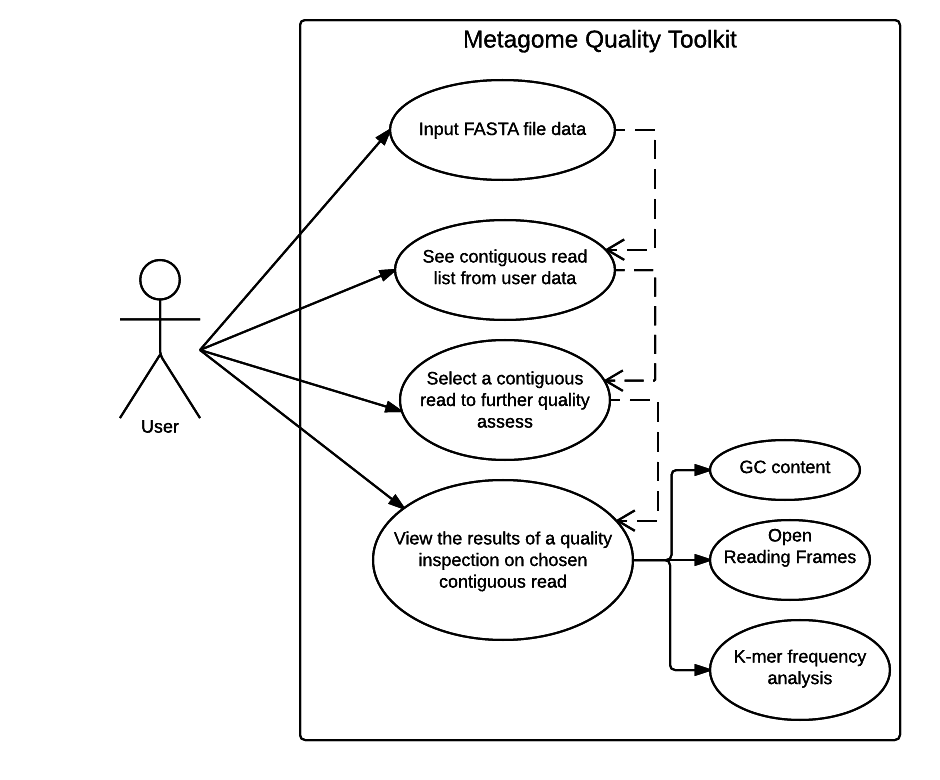
\includegraphics[width=0.5\textwidth]{images/usecase}
\end{figure}

\subsection{Implementation}
Based on the requirements I had selected, I decided that I wanted to write my own software for each functional component. While solutions for each component exists individually, I felt there would be more benefit to a user if I could produce just my own software to support the functionality over requiring them to user third part software in order to use my application too.

Additionally to this, I wanted the technical challenge of writing my own software, and enabling the application to be maintainable and expanded upon in the future rather than relying on third party support applications in order to process a users input. The process of developing the application from scratch would also give me the opportunity to learn more about the domain and technologies for development than just consuming output of other existing applications, even if achieving the end result would take more time.

While I knew the project would come to a close on development at the end of the semester, I also wanted to envision this as a project that could be taken forward in the future to be further developed and maintained. For this reason it also made sense to develop my own application without consuming output from third party software, excluding the FASTA files from an assembler. If one of these third party applications was no longer available or their output changed, it would render my application unusable or require more future modification to adapt to changes by outside sources.

%======== PROCESS ==========

\section{Process}
While my project could well follow a plan driven approach, such as waterfall or the spiral model, I believed that an agile approach would be suitable for building it, as I developed the different techniques through breaking them down into tasks. I chose to use Scrum for my framework, and used aspect of Extreme Programming for my daily development cycle adapted to a one person project. I may also have used a feature driven methodology, as I was aware of the features I wished to implement, however, I believed a Scrum approach with weekly sprint iterations would better suit my work flow.

\subsection{Scrum}
I felt I could produce the best work by working iteratively, using Scrum and having weekly Sprints. A Sprint is -what is a Sprint- and it would be useful to the project because -why is a Sprint useful here-. I held my sprint planning and retrospectives every Tuesday after meeting with my supervisor. 

The Scrum framework had me taking my initial Objectives mentioned in the previous section and turning them into `epic' Stories. Stories are -write about Stories and tasks here, including examples of Sprints-

Task break downs helped me focus on what was important, and gauge what needed to be done and how much effort vs time it would take -include image of whiteboard with task here-. The Scrum framework was naturally adapted to a single person project, as there was no external scum master, client or manager, and these roles were all filled by my own motivation and discipline to be fullfilled.

Daily stand-ups with peers, and how this would help. Adapted from normally discussing Yesterday/Today/Blockers with those who could help, instead to discussing in order to improve motivation and sounding boards.

\subsection{Extreme Programming}
Extreme programming -is what? references and explanation here-. Through choosing XP, I found while I couldn't implement every technique, I took the benefits of Test Driven Development and Refactoring

Test Driven Development is ... it would be useful for iteratively building upon my application, and help with refactoring later. TDD helps with the design of the application, in structure and in what needs to be developed next, and helps with time constraints through forcing only what needs to be developed to be developed and no more. - Include examples of some of my tests here, going red, green, red, green-

Refactoring is... With the knowledge that I wanted my application to be something that could be built upon in the future, refactoring was vital for cleaning up the code structure as I built it with TDD, making it maintainable by others in the future, ensuring that the code is readable and cutting out clutter and duplicate code. While it may be seen as a time consuing and unnecessary task by some, when looking at an application life cycle it is vital to a projects success in the long term.

\subsection{Pomodoro Technique}
Additionally, I found it useful to break my development work into small cycles, using the Pomodoro technique (cite needed), in order to increase my focus and productivity while doing work. The aim of the pomodoro technique is to spend 25 minutes with full focus on the work, and then giving yourself 5 minutes to stop and have a break. They are also useful for keeping track of work done and visually seeing how much time has been invested into the project for the day -include image of pomodoro day here, and link to the website-
Due to the short length of each pomodoro, it was also seen as an effective method for squeezing in work where there was time. By quantifying time into small slots, it made it possible to consider how much time I might have between other events in the day and work out where it could be possible to put in a single pomodoros worth of work, instead of perhaps not working because I felt I did not have the time, or working and eating into other daily activities if I didn't block out the time and be aware of when to stop.

\subsection{Project blog}
While developing my application I kept a blog about my project, any milestones I reached or interesting sections. While I did not designate a particular time to blog, I believed it would be a useful tool in reflecting on the work done when writing this report, something for my supervisor to be able to check upon my progress between meetings and give me the time to reflect on the work done and any upcoming tasks to help me mentally process where the project was in its lifecycle against the planned objects.

% You need to describe briefly the life cycle model or research method that you used. You do not need to write about all of the different process models that you are aware of. Focus on the process model that you have used. It is possible that you needed to adapt an existing process model to suit your project; clearly identify what you used and how you adapted it for your needs.

%\addcontentsline{toc}{chapter}{Development Process}
\chapter{Design}

Talk about UI, Data importing, The way classes are structured, what languages were used, UML, flow diagrams and how the data flows, why does it flow that way. Use Case Diagram

% You should concentrate on the more important aspects of the design. It is essential that an overview is presented before going into detail. As well as describing the design adopted it must also explain what other designs were considered and why they were rejected.

% The design should describe what you expected to do, and might also explain areas that you had to revise after some investigation.

% Typically, for an object-oriented design, the discussion will focus on the choice of objects and classes and the allocation of methods to classes. The use made of reusable components should be described and their source referenced. Particularly important decisions concerning data structures usually affect the architecture of a system and so should be described here.

% How much material you include on detailed design and implementation will depend very much on the nature of the project. It should not be padded out. Think about the significant aspects of your system. For example, describe the design of the user interface if it is a critical aspect of your system, or provide detail about methods and data structures that are not trivial. Do not spend time on long lists of trivial items and repetitive descriptions. If in doubt about what is appropriate, speak to your supervisor.
 
% You should also identify any support tools that you used. You should discuss your choice of implementation tools - programming language, compilers, database management system, program development environment, etc.

% Some example sub-sections may be as follows, but the specific sections are for you to define. 

\section{Overall Architecture}
Evolutionary design. No initial design documents. By using my user stories I knew what tasks needed to be done and considered how would be best to implement them. This lead to the design evolving over time, both in the code structure, classes and user interface. Added functionality as and where needed. Use of prototypes, i.e. ORF Location prototype (show via blog, then show via final result screenshots).

Started by considering what langauge would be appropriate for the processing and display, and at first thought Java would be a good idea. Lead on later to realizing I wanted more than just what Java could do by itself, and chose to make a web serivice, using Java Spring Boot, deployed with Tomcat. I could have instead at this point switched to using Ruby on Rails, but with my prototype code for the GC Content percentage finder done in Java, and without the need for any Active Record, it felt like Java would be the better option. Also portable, as the data processed may be quite large, so Java to allow the application to be run through the JVM on any system (e.g. a Linux HPC) would be appropriate.

OO approach relevant to represent things as Objects. Such as a GC result, ORF Result, etc. Easy to access these items in the browser through thyemleaf as Objects with known names and properties.

\subsection{Choice of technologies}
Why Java instead of Ruby, for example?
Why use Javascript once I decided to use a web service. Because of Plotly and Canvas? Usability? Accessing data. How about how the data is structured in Javascript?
Why did I select plotly and canvas in particular? Fine level control in canvas, ease of use with Plotly, allowing a user far greater control over viewing their charts than I could provide in the time.
Why thymeleaf? very useful for accessing Object data provided by the model. Using fragments for importing sections - Helps remove duplicate code, e.g. for importing the header, and keeping files clean and changing internals of particular charts in their own files, e.g. qualityparameters.html fragment.

\subsection{MVC Framework}
\subsubsection{Model}
Data and structure. ORF sections, GC sections, utility classes and functions, controller access
\subsubsection{View}
Building the view with Javascript and HTML5, using thymeleaf to access data in an OO way.
Choice of designing for the view, let it have the data from the Model, passed from the Controller, and how it deals with displaying the data is completely down to the view. Could develop some parts of the view within the code and pass that to the View, but decided it would be better to instead pass the data as is, and let the view decide on the way of display. This allows the front-end and design of the view to be changed in the future without having to go into the internals of the code base and Model itself to change. Keeping the View and Model separate.
\subsubsection{Controller}
Access through GET and POST methods, validation through Java Spring, response to requests and putting objects into the model to be accessed via thymeleaf, through the controller and put into the view. 

RESTful interface? GET/POST with session parameters. URL is basic 'list' 'toolkit' 'welcome' represents what you get and addressable when needed. (Remind yourself about the principles of REST and talk about them here!!).

\subsubsection{User Input}
FASTA file format - Standard format for assembly data.
Considered File Uploads, and still contains the code for doing this, used for my test files, however, pasting user content was more secure and acceptable for testing. The code for file uploads still exists to be used in revisions to the application.
Data is processed in a FASTA reader, and does these things...
This way of handling the data, returning it to the controller, and then passing it on to the toolkit area of the model to be 'qualityAssessed', where there are the calls to the techniques used. Again, in a future revision and with more techniques, it may be worth while to allow the user to disable or enable particular techniques they are interested in.

User data is not kept by the application, it is stored in a user session that expires once they leave the page. This is handled by Java Spring, and set as a @sessionvariable (..), show an example image of these in the code. If the user does not have their session variables, they are presented with the Error page, so they cannot try and access areas of the application/web service where they currently do not have access or the data to do so.

\subsection{Directory Structure}
Java Code stored in three sections. Main is top level, going down into Domain code, Utility code and Web code. All resources, such as stylesheets, html files and javascript stored under resources folder in static directory. HTML stored as template .html files for use by Thymeleaf, Javascript broken up into multiple files based on where they are used (toolkit.js, list.js) and their functions (orf-chart.js, gc-chart.js). Separating out the files this way improves readability and maintainability. Keeping things isolated and simple.

Using MVC - What is MVC - What else did I consider? Did I think about using a command line tool, why no good? Report output. What about using something not a web service? Why did I choose to do a web service instead?

Started working on Java code with the intention of making a GUI that would do the things. Decided


\subsection{QualitySummary}
Results returned in a QualitySummary object. Object contains references to GcResult and OpenReadingFrameResult. Option to have these two implement an interface that might be called QualityResults, and have just an array of QualityResults. This would allow us to add any type of result without needing to know what is in there. However, chose not to do this as considering the way in which we serve the view results and them being so tightly coupled to the view, didn't seem necessary through the evolutionary design. Aware that in the future if we allowed a user to select what type of processing they wish to use, this technique would be very useful to implement, and only serve up the results tabs that they wish to see. However, as stated, evolutionary design through TDD so wasn't yet necessary.

Show how the design is structured. How do we go from the file to the processing? Why did I do it this way? What were my initial designs.
Considering ORFS - Result is an ArrayList of the OpenReadingFrameLocations, why this way? First looking at just 'the longest', then prototyping it out to find one in each frame, then breaking it out into finding Start/Stop Codons and 'stitiching' them together where appropriate.

\section{User Interface}
Framework mock ups of the user interface. Logo for kicks.

- Input form, why is it this way?
- List - Displaying each contig, why, framework, drop downs
- Paramters - Why did I pick these Paramters, what use are these for the user? Why GC content windows and what size is reasonable? Can demonstrate domain knowledge about the choice of parameters. Up to the user, allowing them to put in stupid numbers, but their results are their own.
- GC Chart - Why does it look like this - Choice of standard deviation and mean, why? What use does this actually have  in showing the user error areas? What about just visually seeing the data? Show the screenshots of areas out of GC content threshold, show the areas where obvious chimera (50/50 example)
- ORF Location - Why did I develop it to look like this? Representing each of the 6 frames, demonstrate the reverse frames are displayed in the correct direction. How did I achieve this and why display it this way and the inner detail? Other approaches? What about the NCBIs version? Ability to click. Also the list? Why have both? They're both useful to have, as a user may want to look at the shortest ORF Location but not be sure where it is even when they read what frame it is. Likewise they may want to see where an ORF Location lies in the list organized into longest to shortest. Why organized into length. Useful to the user to get an idea to further inspect.
- Superframe - What is it and why did I consider it. Showing overlaps and where the Red areas may be areas of errors and what to look for. The explanation of it, why explain it this way? 

\section{Support Tools}
For writing the code, I used JetBrains IntelliJ IDE (screenshot of IDE window with some code). This included writing all the code, Java, HTML, CSS, Javascript, ThymeLeaf and any additional properties for setting up Spring Boot. Useful for text highlighting, debugging the code, and tied into my version control, using Git and hosted on GitHub. (screenshot of commits)
\subsection{Version Control}
Using version control to keep a repository of code in case of lost data in event of hardware crash or software corruption. GitHub decent choice, already had a repository on there and Git supported in IntelliJ IDE. In addition, every time I check in, I used continuous integration with CodeShip, allowing me to receive e-mails any time I made a commit to my repo that didn't pass the tests written. Very helpful in discovering issues with failing builds when checking in a change and forgetting to update tests or breaking previously written code as the design changed (show screenshot of failing/passing builds from CodeShip).
\chapter{Implementation}
This chapter serves to discuss the implementation specifics of the design of my application, including the development environment and any issues I encountered in implementing the features set out in my project objectives.

\section{Development Environment}
The application was developed primarily on a Fujitsu Lifebook A series with an Intel i5-3230M CPU @ 2.60GHz processor, 4GB of RAM and running Windows 10. The code was developed using Jet Brains IntelliJ IDE and Google Chrome developer console.

\section{Features}
\subsection{Reading User Input}
\subsubsection{Implementation}
The user input was one of the first parts of the application to be implemented, and consisted of reading in a .fa FASTA file and just outputting the content of the file to the console and return it from the method to be tested against with automated unit tests. It was developed further to extract out the header, checking that it began with the `\textgreater ' character and then every other line was included as part of that contig. 

Originally it dealt with only one contig at a time, but was then expanded to be able to read in a full list of contigs and separate them based on where the header line starts. The code was eventually modified so that the user could paste data, that would be broken into components and processed in the same way. This was for the pasting of the user data rather than file upload, as I decided I would rather have pasted data than uploads for the current state of the application.

\begin{figure}[H]
\centering
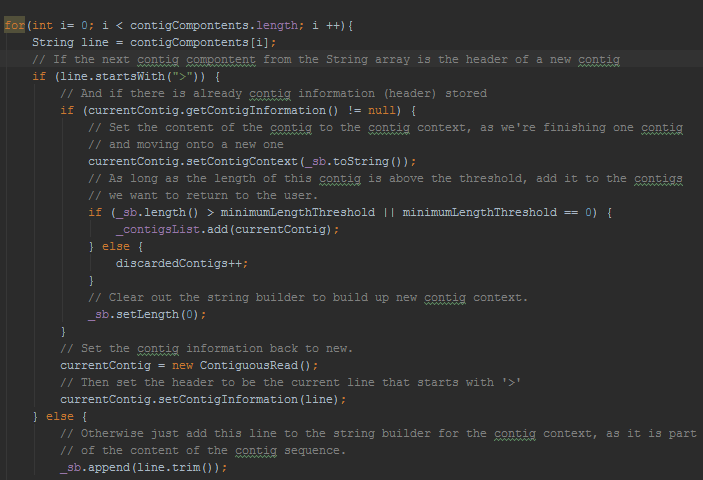
\includegraphics[width=0.9\textwidth]{images/readuserdata}
\caption{Part of the code for reading in a users data when they have pasted it into the text area of the web service. Deals with creating new ContiguousRead objects and adding them to a ContigResult every time it finds a new header for a contig (or reaches the end of the input).}
\end{figure}

\subsubsection{Issues}
It took some time to deal with the formatting of the file and knowing when one contiguous read starts and one ends. There was some issue with the escape/return characters in the dealing of pasted content by a user, but this was solved by breaking the pasted content into an array of its components.

While not an issue as such, the original version of the application would carry out the quality assessment of each contig as and when they were read in, to avoid holding too much data in memory. As the design evolved this was no longer a possibility, as it didn't allow the user to see their contigs before they were processed, or do any additional inspection on the contigs without holding the entire user data submitted in memory and going through it a second time upon an inspection request to find the contig they wanted. This option is still a possibility, but is an optimization aspect that wasn't in scope for the project. Additionally, the separation of responsibilities is better in this version of the code after being refactored from the time when the read class both read and assessed the contigs.

It did take longer to implement this than I had anticipated due to me changing from file reading to user pasting, and trying to find contig start and ends to read in the data versus read and assess at the same time.

\subsection{Counting GC Content \& Percentage}
\subsubsection{Implementation}
Counting the GC content of the application involved breaking up the contig characters into sizes based on the set window length by the user, then working out the percentage of G and C characters in each of those windows. Each part of the contig that is split is put into a `GcWindow' object, that has methods for counting the number of G and C characters within it.

\begin{figure}[H]
\centering
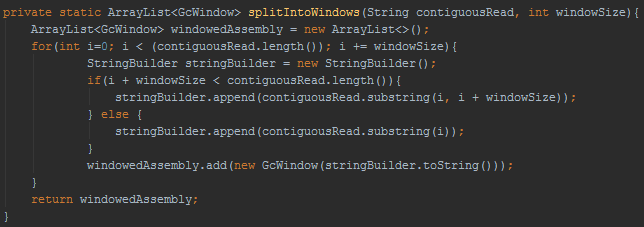
\includegraphics[width=0.9\textwidth]{images/splitgcwindows}
\caption{The code for splitting a contiguous read into windows available for calculating the GC content window percentages.}
\end{figure}

Once split, the GcWindows are passed to have their percentages calculated and added to an ArrayList of Doubles This is used for calculation with the mean, standard deviation and for returning results to the user for use in the View.

\begin{figure}[H]
\centering
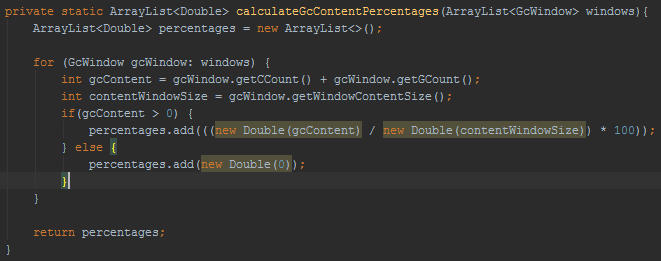
\includegraphics[width=0.9\textwidth]{images/calcgcpercentage}
\caption{The code for calculating the GC content percentages for each window passed into the method.}
\end{figure}

\subsubsection{Issues}
In principle this is, and was, an easy task, yet took me longer to complete because my domain knowledge was still somewhat lacking and I got caught up on the little details that kept me from progressing, even though I didn't need to know of them or use them in the process of working out the GC content windows. Overall there were no issues with the implementation once I got my head around why it was worth doing this and how it should be presented as a quality measure to the user.

\subsection{Displaying GC Content percentage}
\subsubsection{Implementation}
I began to attempt to implement GC content viewing with Plotly.js right from the beginning, and so I had a prototype up and running fairly quickly where I manually took the results from the console output of the Java application and pasted them into the final containing my Plotly.js prototype to be used as data. 

Next I worked this in with Thymeleaf to get the results directly from my Java application, then turned them into JavaScript and used the data from that for the chart. The x axis labeling for the chart is manually created in order to represent where the GC window for each bar starts and finishes. The earlier design had window numbers along the x-axis, populated by Plotly.js. These were of no use to a user though, as if they wanted to find out what GC window they were looking at they would have to manually work out where the window started and ended from their window size multiplied by the window number of interest.

\begin{figure}[H]
\centering
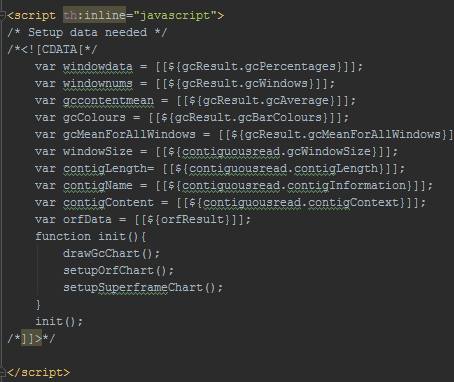
\includegraphics[width=0.6\textwidth]{images/thymeleafdata}
\caption{Extracting the data from the Model, provided by the Controller to the View, using Thymeleaf's inline tag to be able to use CDATA to convert the Thymeleaf extracts into JavaScript.}
\end{figure}

The red bars of the GC chart displaying where the percentage of a window is over or under the threshold of the mean of all GC window percentages was implemented as a useful aid to the user, and the colours are set in the Model rather than made in the View. The reasoning for this was to implement a system that would provided the View with what it needed and not needing the View to calculate anything, only consume the values (in this case the GC window data and RGB data) to display results.

\begin{figure}[H]
\centering
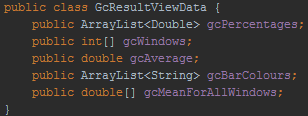
\includegraphics[width=0.6\textwidth]{images/gcviewdata}
\caption{`GcContentViewData', the object provided to the View in order to display the GC content data to the user.}
\end{figure}

The final thing to add was the Mean line. This is just displaying to the user where the mean of all the GC windows lie, and helps with the visualization of if any windows of their contiguous read look like they might have issues.
\subsubsection{Issues}
The main issue I had with displaying the GC content percentages with Plotly.js was getting data to actually display as I was unfamiliar with Plotly.js and Thymeleaf once I started using Spring Boot. Thymeleaf makes getting data from the Objects in the Model very easy and simple, but since I was trying to integrate two technologies together that I had never used before, it took some time to find the right way of accessing the data from my Object through Thymeleaf, into JavaScript and then the correct format for use by Plotly.js.

The next issue was trying to get the line for the Mean to show. The way I got this to work was using an additional data input for the same chart as displaying the GC content window bars and having the same number of data points as there are GC windows, where each data point is the mean number, in order to get the chart to display a line across the entire chart to match the GC windows.

\subsection{Finding Open Reading Frames}
\subsubsection{Implementation}
The implementation of Open Reading Frames happened in a few steps, with the design and code evolving as I understood more what they were and how best to present the results. At first, I was only finding a single, longest ORF Location, as I did not fully comprehend what an ORF was. This was just looking at a contig and finding the first start Codon of ATG and the last stop Codon of TAG/TAA/TGA. Once I understood them though, the process became about how to find whatever ORF Locations I could. Using Test Driven Development was extremely useful for this step, as I wrote tests for finding specific ORF Locations in small sequences I created myself and ran the code against them.

After a number of attempts at trying to find the ORF Locations within a contig frame, I settled on a method of going through the entire frame, breaking it up into characters of 3 and only keeping the start and stop Codons in lists of each. Each Codon was stored with data about where it starts and ends, in order to be able to later reconstruct the contig between a start and stop Codon based on the character positions.

\begin{figure}[H]
\centering
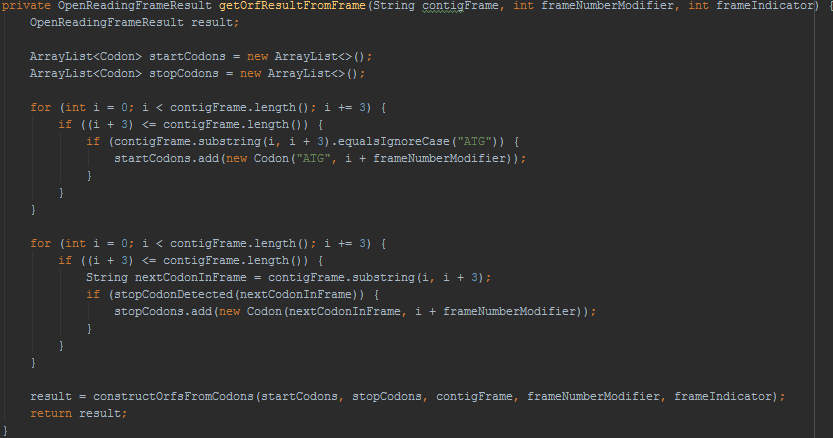
\includegraphics[width=0.9\textwidth]{images/orffind2}
\caption{Finding all of the start and stop Codons from within the passed frame from the contig.}
\end{figure}


Each frame is separated by creating a substring of the original contiguous read, removing 0, 1 and then 2 characters for the first three frames, and the same for the reverse frames but with the contiguous read sequence reversed with the opposing base pair of each character used. 

\begin{figure}[H]
\centering
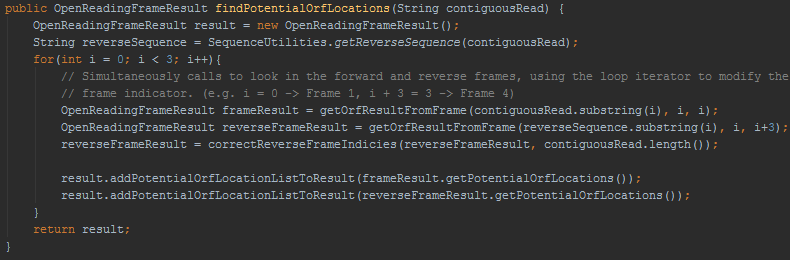
\includegraphics[width=0.9\textwidth]{images/orffind1}
\caption{Extracting each frame and calling to run the ORF Finding process.}
\end{figure}

For each ORF Location found in a reverse frame, the start and stop indexes are swapped, representing that what is the `Start' of an ORF Location is actually closer to the end of the contiguous read. This is so that it can be displayed appropriately in the View, and match up with the proper direction with the forward frames.

\begin{figure}[H]
\centering
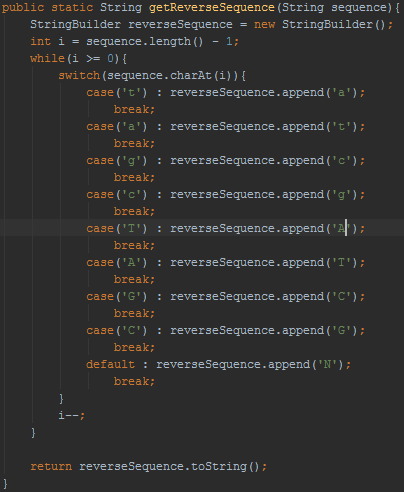
\includegraphics[width=0.6\textwidth]{images/orffind4}
\caption{Getting the base pair characters of a reverse frame is as simple as a switch statement and building the reversed contig from back to front.}
\end{figure}

Through this process, it made it possible to find which Codons came before and after which within the contiguous read in order to find which would construct the longest ORF Locations, which Start Codons were redundant (as they were between an earlier start Codon and the next Stop Codon), and in my first completed version of the algorithm, where the last Stop Codon before the next Start Codon was.

At this time, I still had a misunderstanding about protein coding regions, in that I believed the end of an ORF Location was at the last stop Codon before the next start Codon, when in fact it should have been the first stop Codon it reaches is the end of the current Codon. This was a simple fix though as it just involved removing a section of my code and fixing my tests.

\begin{figure}[H]
\centering
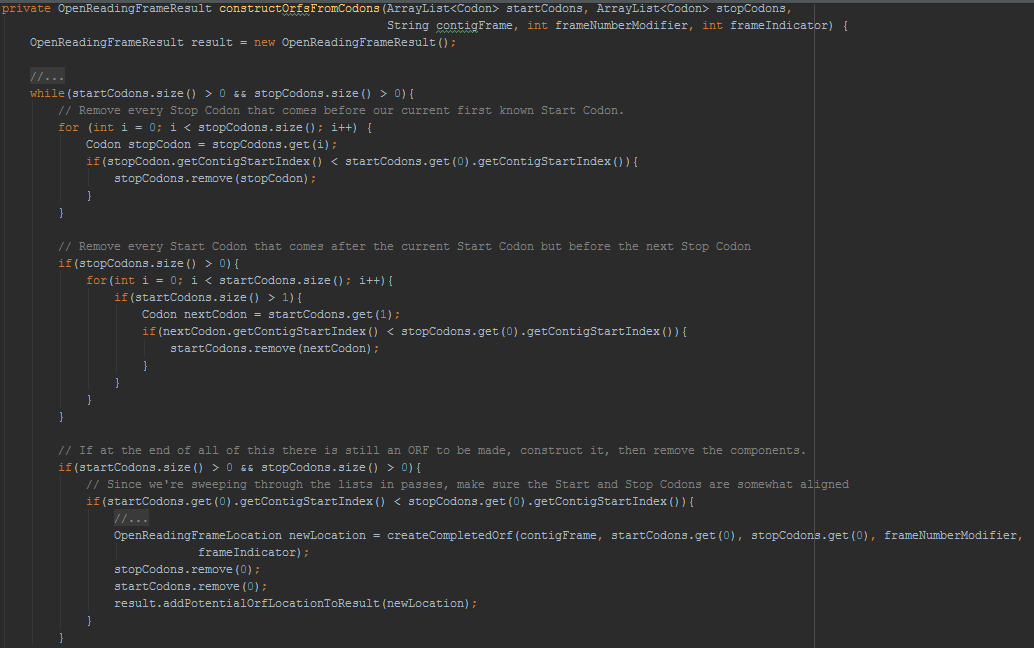
\includegraphics[width=0.9\textwidth]{images/orffind3}
\caption{`Zipping' together ORF Locations from start and stop Codons within the frame.}
\end{figure}

Once each frame has been processed to find the ORF Locations within them, the results of each frame are combined together in a single OpenReadingFrameResult. Each ORF Location is aware of what frame it belongs to, and so combining them all into one result doesn't make a difference when determining what ORF Location belongs where.

\subsubsection{Issues}
The two main issues with implementing the Open Reading Frame finding algorithms were my lack of understanding of what they were when I began, leading to the second issue of implementing more than was necessary. It took me longer than I had anticipated to implement the code for finding ORF Locations because I believed I had the additional requirement task of finding the last stop Codon before the next start Codon, where every stop Codon between the initial start Codon and that last stop Codon was to be included in the ORF Location but ignored as an actual start and stop.

Thinking up how to do this algorithmically took some planning and time, and eventually I came to the conclusion of finding all start and stop Codons and then running a while loop, checking that there was at least 1 of each left in each list to make an ORF Location, where the Start came after the Stop (for reverse frames, this logic still applies as the indexes are only reverse after the ORF Locations have been constructed) and then carrying out a number of conditional checks to remove any start and stop Codons that came between the longest ORF that could possibly be made.

Once I had realized this was erroneous and the first stop Codon encountered is the actual end of an ORF Location and not to continue, it was too late to recover any time and I just had to remove the code that caused the issue and rewrite my tests to match the actual expected outcome. Aside this, once I designed the code based around the `zipping' of start and stop Codons together, the implementation was relatively simple, using unit tests to ensure I was correctly implementing the algorithm for expected results.

\subsection{Displaying ORF Locations}
\subsubsection{Implementation}
The first part of the ORF Location displaying for the View takes place in the Controller, where it strips away ORF Locations under minimum length threshold set by the user and then sorts all ORF Locations by length using a comparison method. The display of the ORF Locations in their particular frames is done using HTML5 Canvas, one for each frame. As each ORF Location holds an integer value representing what frame it belongs to, when painting the canvases it is a simple matter finding the correct context  for the particular frame from an array of canvas contexts
\begin{verbatim}
var currentContext = contextList[orfData[i].frameIndicator];
\end{verbatim}
Reverse and forward frame ORF Locations are painted in the same way, except the start and stop indexes are swapped for reverse frames. Likewise, for the highlighted ORF Location to be painted, the only difference is that the current highlighted frame is stored in a global variable (updated any time an ORF Location is clicked in the list or on a frame) and when re-painting the frame canvases and iterating through the list of ORF Locations, when the loop reaches that ORF Location the fill colour is set to be different than every other ORF Location.

Finding a click within a canvas frame is as simple as checking if the click is horizontally within a frame location by calculating where the start and stop points of all the ORF Locations (with that frame in particular) are and if the click falls within one of the the ORF Locations.

\begin{figure}[H]
\centering
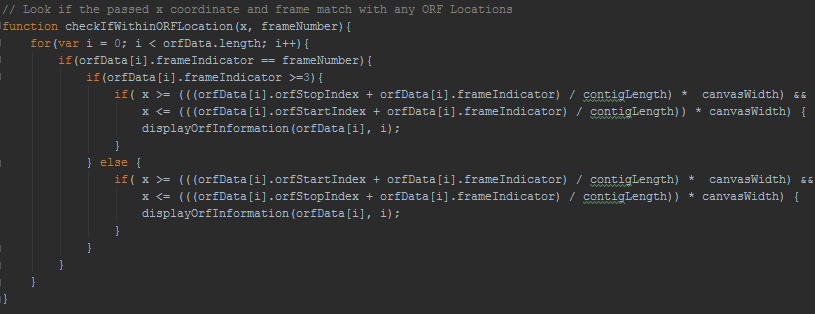
\includegraphics[width=0.9\textwidth]{images/orfdisplay1}
\caption{Finding if a click if within an ORF Location is as simple as going through the list of ORF Locations, only checking against those within the same frame as the click, then looking at whether the click is within the start and stop points of an ORF Location within the canvas, based on the size and location of where it was painted (for reverse frames, the start and stop points are swapped, as reverse frames are displayed in the same direction as forward frames, with the indexes in the right order for a reverse frame).}
\end{figure}

When an ORF Location is clicked to be viewed in more detail, the characters within that sequence needed to be formatted to be able to be reasonably displayed. This process took some time to build, and through refactoring was re-written twice over until I found a result that was reasonably fast at formatting and worked the way I wanted it to. This is that it highlighted every start and stop Codon within a sequence, split the characters into groups of 3, every 15 groups of 3, a new line is to be created and where the start of the line has the index within the contiguous read where that line of the ORF Location begins.

\begin{figure}[H]
\centering
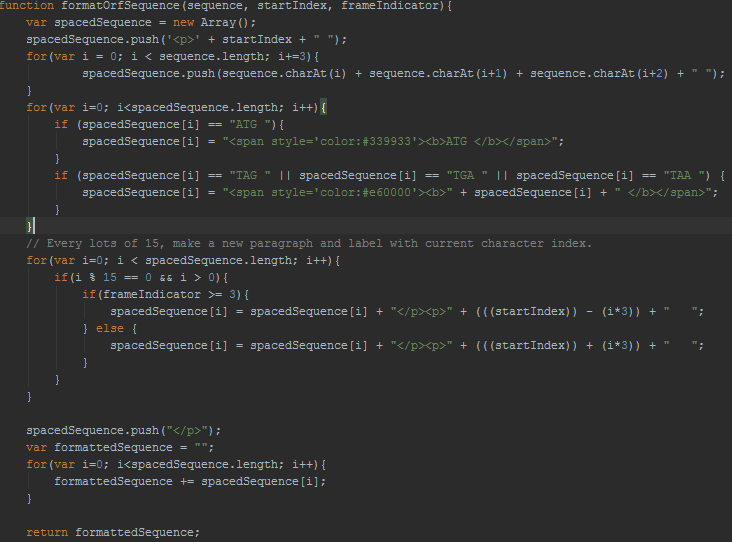
\includegraphics[width=0.9\textwidth]{images/orfdisplay3}
\caption{Formatting the characters from within an ORF Location into HTML tags to display the data in the way I wanted it to be designed, then inserting it into the div for displaying ORF Location information within the page.}
\end{figure}

\subsubsection{Issues}
When formatting the ORF Location characters into the list, I found I kept having results where the newline break would be incorrect, or not all of the start Codons were highlighted. This issue was because the way I built the formatted text was by adding text into an array, and then breaking up the text to add newlines whenever the array had a remainder of zero when divided by 15. This meant that it was including the indicator of what index the line of the ORF Location was on as part of the calculation. The result was that the line would be split incorrectly. Once I changed how the formatting was done and included the character index as part of the first set of characters of each line, the calculation worked correctly for splitting the lines where I wanted them to be split.

Although not an issue as such, my first version of drawing the canvas frames involved a single canvas. While the displayed result was the same, it meant that the detecting of user clicks within ORF Location algorithm took longer to process as it had to determine which frame the user was clicking on and then find if it was within an ORF Location. Additionally, having it all in one canvas made the formatting of the canvas results on the page a little more challenging as I couldn't place values (like the frame indicator) exactly next to each frame without painting them within the canvas.

By just splitting the single canvas into 6 different canvases, one for each frame, it allowed me to easily surround the canvas elements with text for frame indicators and cut down on the code for detecting where and what the user was clicking on within each frame, as shown in the implementation of the click detection above in the section above.

\subsection{Superframe Comparisson}
\subsubsection{Implementation}
Implementing the Superframe was a relatively simple procedure as all of the data required, and part of the code, had already been done within the GC content and ORF charts. Since the Superframe just displays both of these together, it was simply overlaying the 6 frames together and painting on the GC content windows that were out of the threshold (above it, not below) and painting lines to represent the breaks between windows. The algorithm for detecting and highlighting user clicks within windows is also much the same as the code user for the ORF Location clicks and highlighting, just modified to detect within windows rather than within the frames.

The canvas is set up so that it could also be used with other future techniques from within windows, such as k-mer frequency analysis results, and be a tab page where any comparison or overall results could be displayed.
\subsubsection{Issues}
There were no issues implementing this content as the code had mostly been done previously. The main challenge was trying to think of a good way of displaying to the user where there might be potential issues, and giving them a report on the quality. What the application does is just displays them this overlay of the techniques used right now and leaves them to come up with their own decision.

It would be nice in future to be able to expand on this and perhaps be able to truly give the user a report that tells them where there are good or bad areas of their data, instead of making them infer it for themselves through this chart, but without additional techniques this is a challenging prospect.

\subsection{Implementation Review}
During implementation, I found that GC Content percentage and ORF Location finding took a lot longer than expected, especially considering that I implemented an additional part of ORF Location finding that wasn't needed, and refactored it 3 times until I reached the point where it correctly found them.

The user interface design and coding to format it also took a lot longer than I had originally anticipated. I wanted to present the information in a clean and useful way, without cluttering the page, and a number of redesigned happened due to the underlying code evolving over time to meet the requirements. Getting used to Thymeleaf and how it took the data from the Objects took a while to get used to, too, as I was unfamiliar with Spring Boot and Thymeleaf and wasn't sure how I was adding the data to the Model and then not clear on how it accessed it, or how it was used in form submissions.

The Superframe also needs additional consideration. A lot of the quality assessment is still on the user to look at the produced reports and their content to consider whether they themselves feel their assembly file is good or not through factors highlighted by my application. 

Overall, these issues and lack of understandings delayed me to the point where I didn't have time to implement k-mer frequency analysis or any of the `nice to have' features, and there are certainly areas of the current implementation where I feel bits are lacking, such as file upload, verbose logging and validation and the aforementioned Superframe. What I have got working though, I feel is of decent quality, my process of iterative development and design evolution with prototyping worked quite well and the requirements for those sections are fulfilled.

% The implementation should look at any issues you encountered as you tried to implement your design. During the work, you might have found that elements of your design were unnecessary or overly complex; perhaps third party libraries were available that simplified some of the functions that you intended to implement. If things were easier in some areas, then how did you adapt your project to take account of your findings?

% It is more likely that things were more complex than you first thought. In particular, were there any problems or difficulties that you found during implementation that you had to address? Did such problems simply delay you or were they more significant? 

% You can conclude this section by reviewing the end of the implementation stage against the planned requirements. 

\chapter{Testing}

% Detailed descriptions of every test case are definitely not what is required here. What is important is to show that you adopted a sensible strategy that was, in principle, capable of testing the system adequately even if you did not have the time to test the system fully.

% Have you tested your system on �real users�? For example, if your system is supposed to solve a problem for a business, then it would be appropriate to present your approach to involve the users in the testing process and to record the results that you obtained. Depending on the level of detail, it is likely that you would put any detailed results in an appendix.

% The following sections indicate some areas you might include. Other sections may be more appropriate to your project. 

\section{Overall Approach to Testing}
My approach to testing was using Test Driven Development and refactoring, taking note from XP practices, ensuring that I only developed as much as was required to make tests pass based upon my requriements for eachi part of the applications intended functionality. The aim was to have as many tests automated as possible, as this would allow me to test frequently and reliably and tie into testing everytime I checked into my Git repository with CodeShip's continuous integration of my code. Where automation could not be carried out, I created test files and used a test table to determine whether my application met the requirements I could test against.

%=== Up to here ===

\section{Automated Testing}
\subsection{Unit Tests}
Writing unit tests before writing any functional code to match against was very useful, allowing me to develop code againsts the tests, written one by one, so that I would not develop any more than necessary. This made is so that what was developed fit the requirements, as the tests written before the code were based upon the exact specifications of the requirements. Refactoring the code after each test kept my design evolving and improving maintainability and simplicity to remove duplicate and unnecessary code.

\begin{figure}[H]
\centering
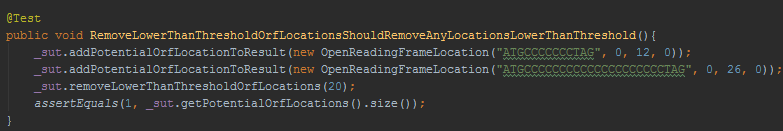
\includegraphics[width=0.9\textwidth]{images/unittestexample}
\caption{An example of a unit test used in my application.}
\end{figure}

Each unit test was made to only carry out one function check at a time, and the naming of each test reflected what the functionality of the system part under test should do. It is for this reason that the item under test is called `sut', system under test, and each test is named with a convention that has a `should' clause in the name, to demonstrated that the function called should produce particular expected results.

\begin{figure}[H]
\centering
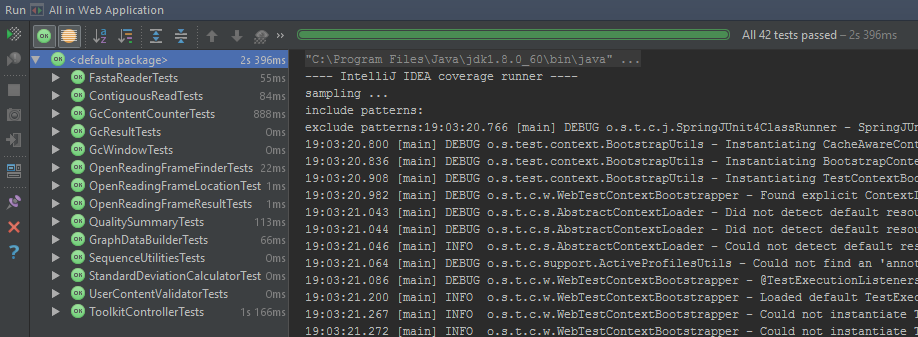
\includegraphics[width=0.9\textwidth]{images/unittestsuccess}
\caption{Results of running the set of unit tests developed for the application.}
\end{figure}

IntelliJ gave  me the tools to run my unit tests with coverage, allowing me to see how much of my code was actually tested against. In the figure below it can be seen that most of my methods were covered. Those methods that were not covered I chose not to test against, as they are mostly setters and getters with no further functionality. In practice, it would perhaps be best to test against these too, in case for some reason the way a value is set or retrieved had to take into account some processing.

\begin{figure}[H]
\centering
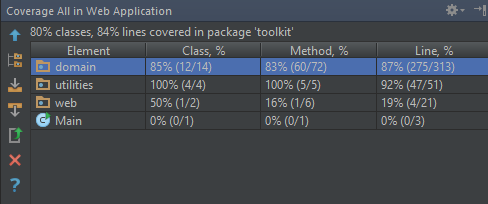
\includegraphics[width=0.9\textwidth]{images/testcoverage1}
\caption{The test coverage of my unit tests over the developed application code.}
\end{figure}

\begin{figure}[H]
\centering
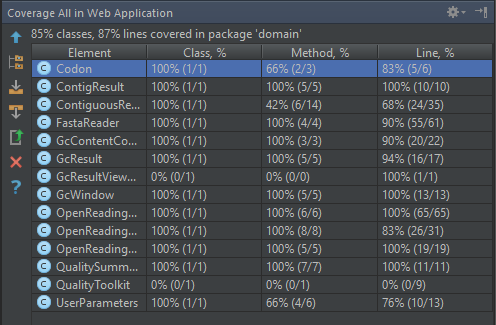
\includegraphics[width=0.9\textwidth]{images/testcoverage2}
\caption{The test coverage of my unit tests over the developed application code, broken down for each class.}
\end{figure}

\subsection{User Interface Testing}
For testing the user interface, I used Chrome's Developer Tools for checking the correct running of the JavaScript, and debugging the code as it ran on loading of the page. I also confirmed that each of my pages loaded and functioned correctly in Google Chrome, Firefox and Microsoft Edge.

\begin{figure}[H]
    \centering
    \begin{subfigure}[b]{0.4\textwidth}
        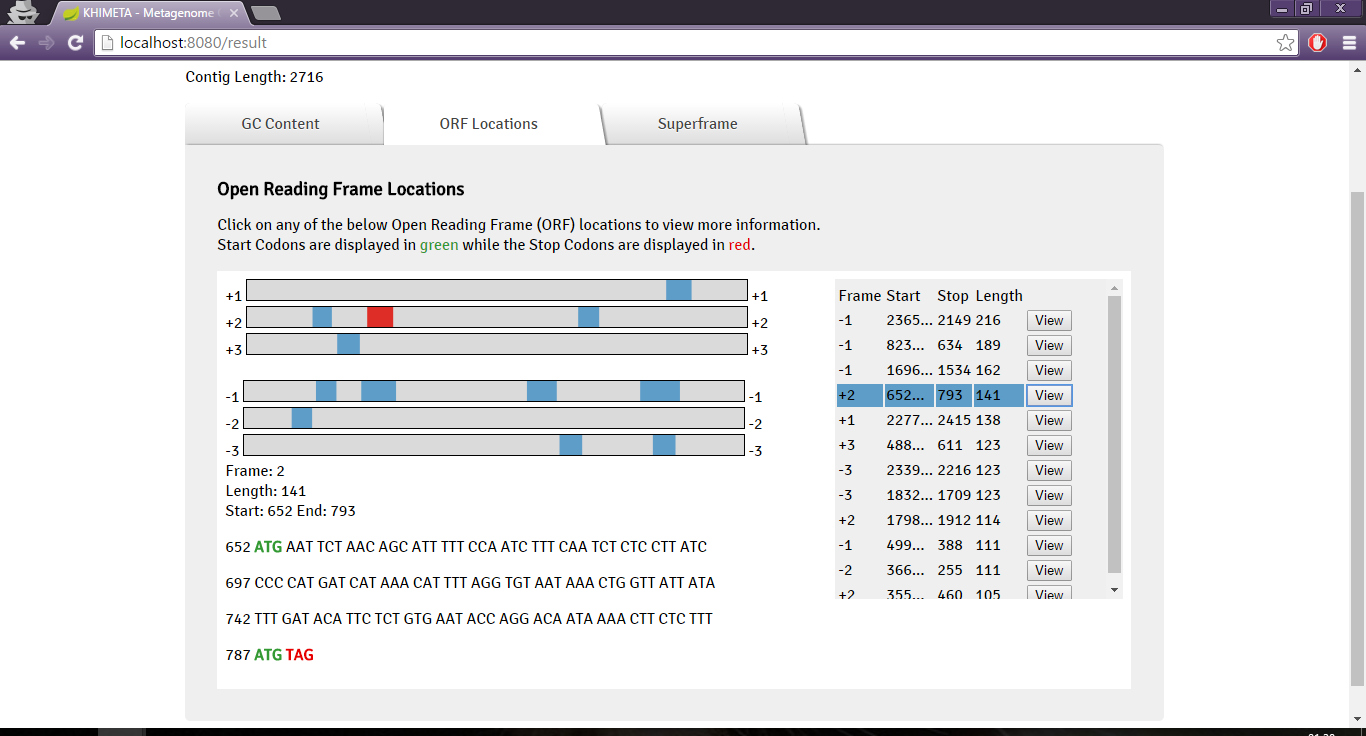
\includegraphics[width=\textwidth]{images/browserchrome}
        \caption{Google Chrome.}
    \end{subfigure}
    ~ %add desired spacing between images, e. g. ~, \quad, \qquad, \hfill etc. 
      %(or a blank line to force the subfigure onto a new line)
    \begin{subfigure}[b]{0.4\textwidth}
        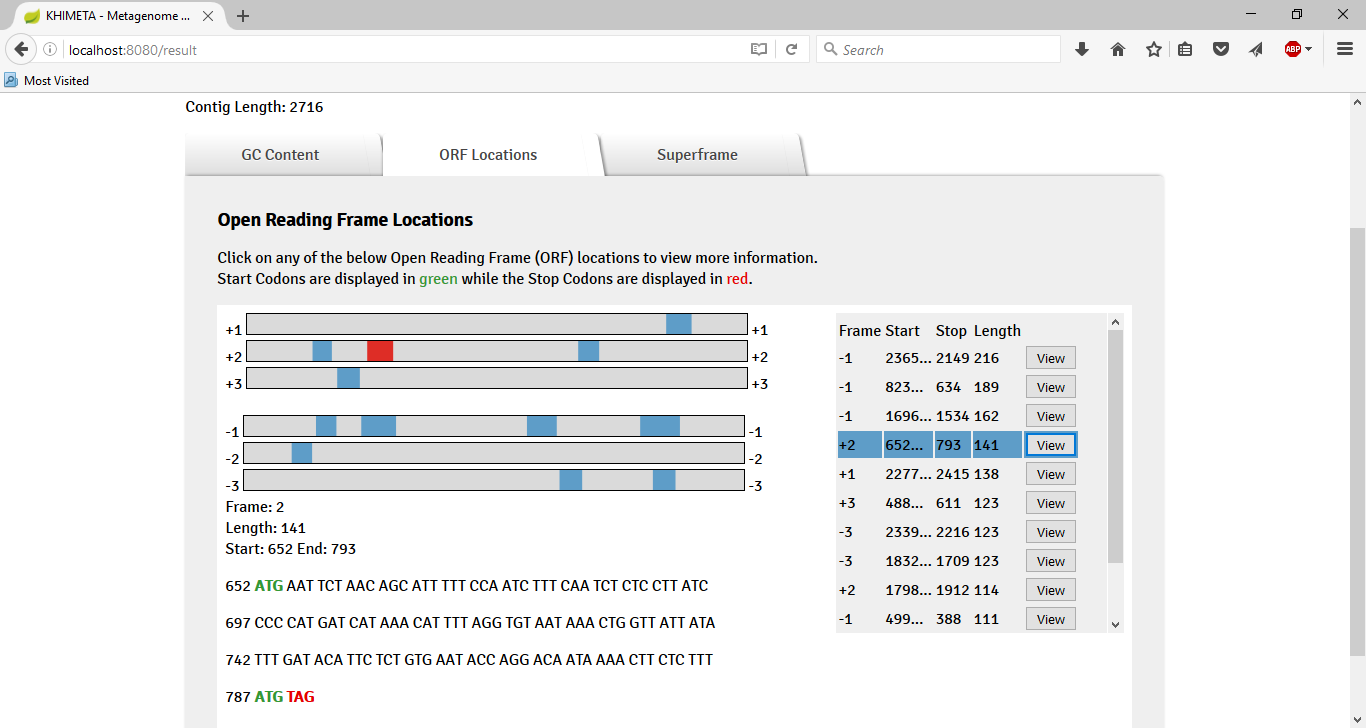
\includegraphics[width=\textwidth]{images/browserffox}
        \caption{Firefox.}
    \end{subfigure}
    ~ %add desired spacing between images, e. g. ~, \quad, \qquad, \hfill etc. 
    %(or a blank line to force the subfigure onto a new line)
    \begin{subfigure}[b]{0.4\textwidth}
        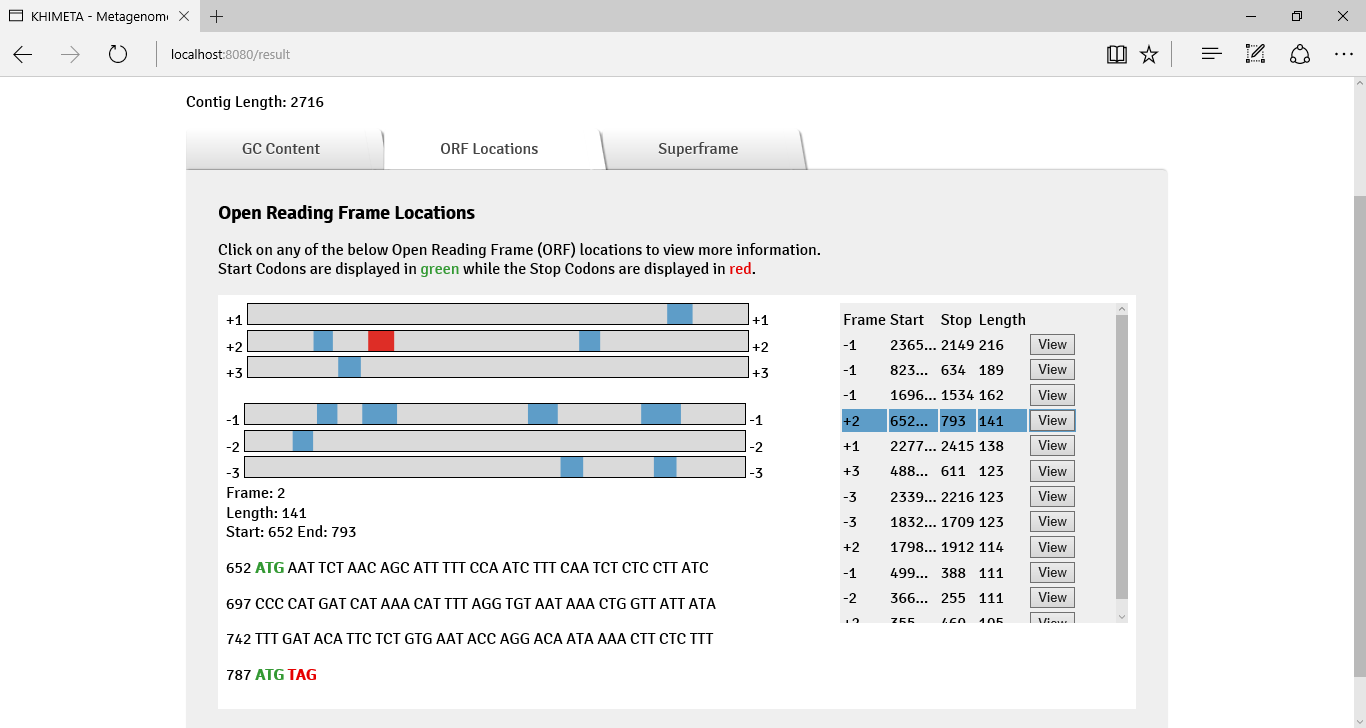
\includegraphics[width=\textwidth]{images/browseredge}
        \caption{Microsoft Edge}
    \end{subfigure}
    \caption{The same page and results from the application shown in different modern browsers.}
\end{figure}

For testing the speed performance of the web pages of the applications loading time, I used YSlow\cite{yslow} which runs a number of checks on the page setup and loading speed to return a report about whether a page loads quickly or slowly, and how it could be improved.

\begin{figure}[H]
\centering
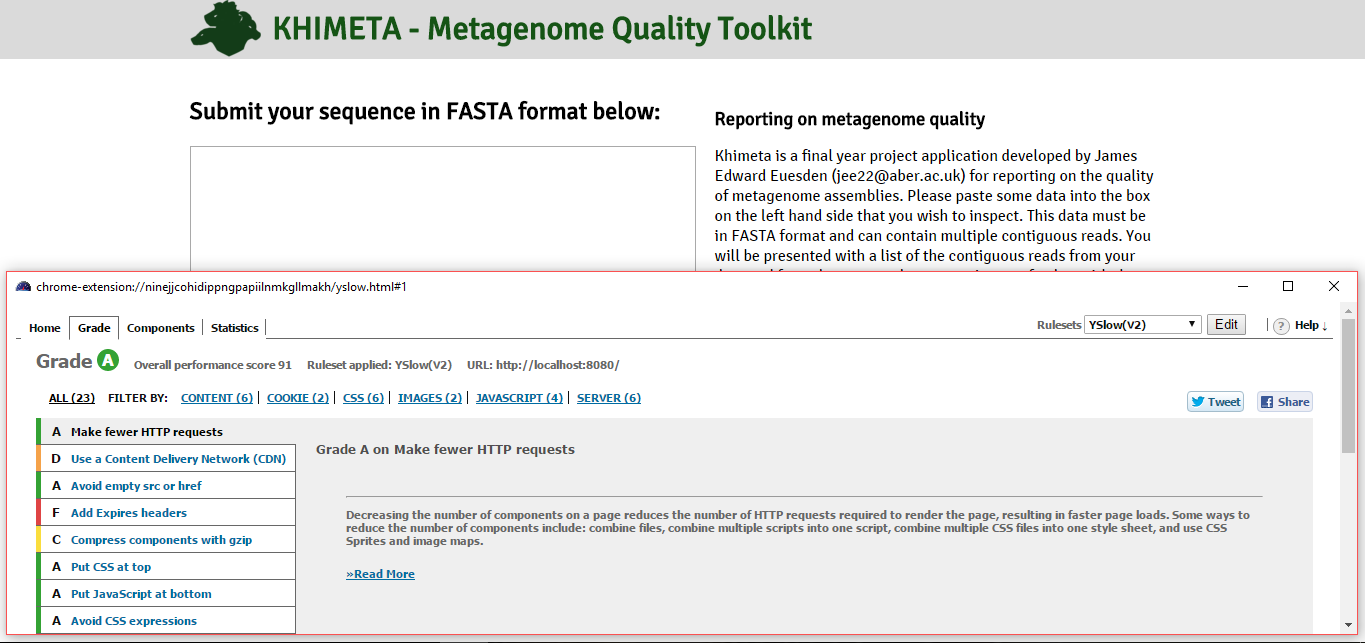
\includegraphics[width=0.8\textwidth]{images/yslowpage1}
\caption{YSlow report after running on the Welcome page.}
\end{figure}

\begin{figure}[H]
\centering
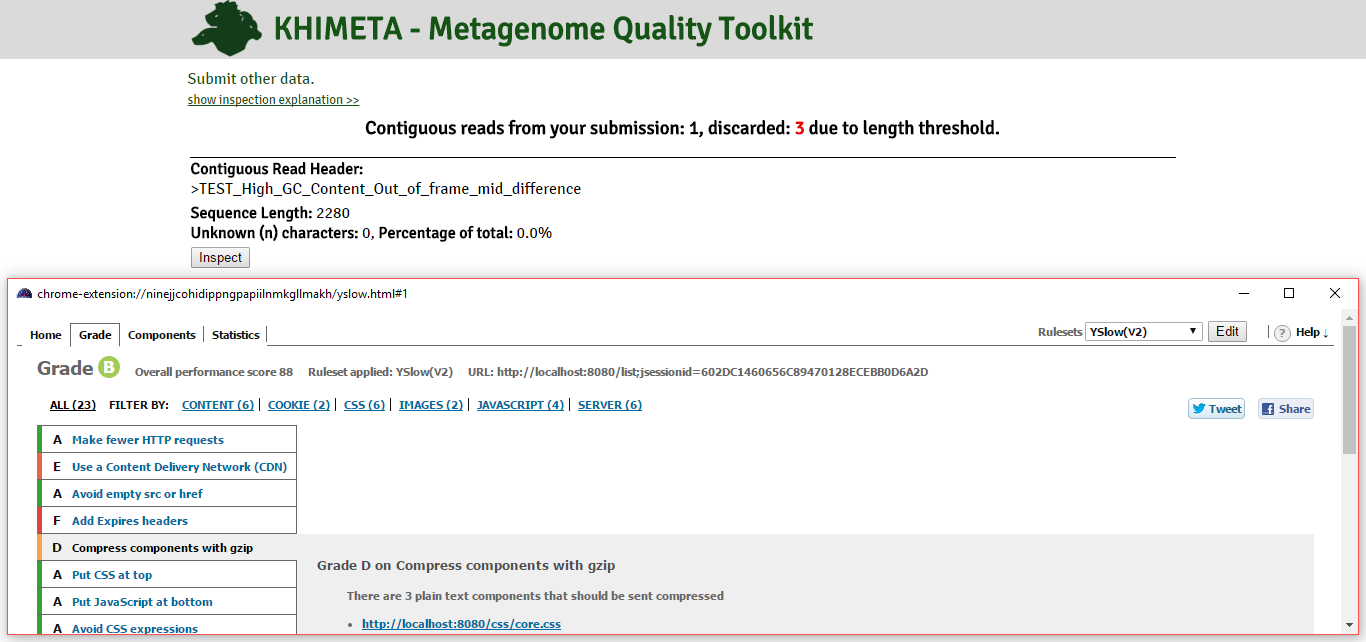
\includegraphics[width=0.8\textwidth]{images/yslowpage2}
\caption{YSlow report after running on the List page.}
\end{figure}

\begin{figure}[H]
\centering
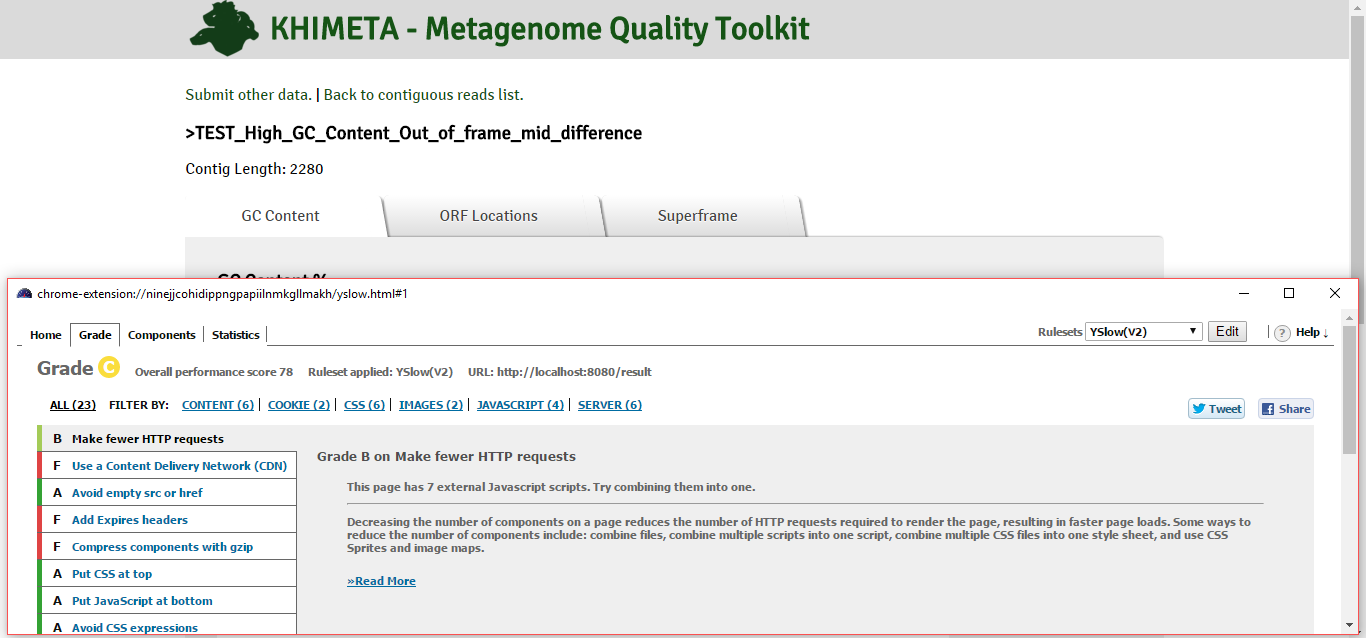
\includegraphics[width=0.8\textwidth]{images/yslowpage3}
\caption{YSlow report after running on the Results page.}
\end{figure}

My results showed me that for the most part there was not much I could do to improve my application outside adding expiry headers to some session variables and implementing a Content Delivery Network (CDN), which was far outisde the scope of the project.

\subsection{Manual Testing}
A number of artificial files were created in order to be used for testing. Some of these were used in automated tests, such as checking for a files existence and possibility of being read, or throwing exceptions when a test file did not exist while other files were for running manually, either being entirely artificial and checking for individual expected behavours, or composed of actual data from multiple species that I manually split and combined together to view the results of. The completely artificial file data is included in the appendices. While the results of the mixed real species data is not included, the results of one very obvious combining of species can be seen in the figure below.

\begin{figure}[H]
\centering
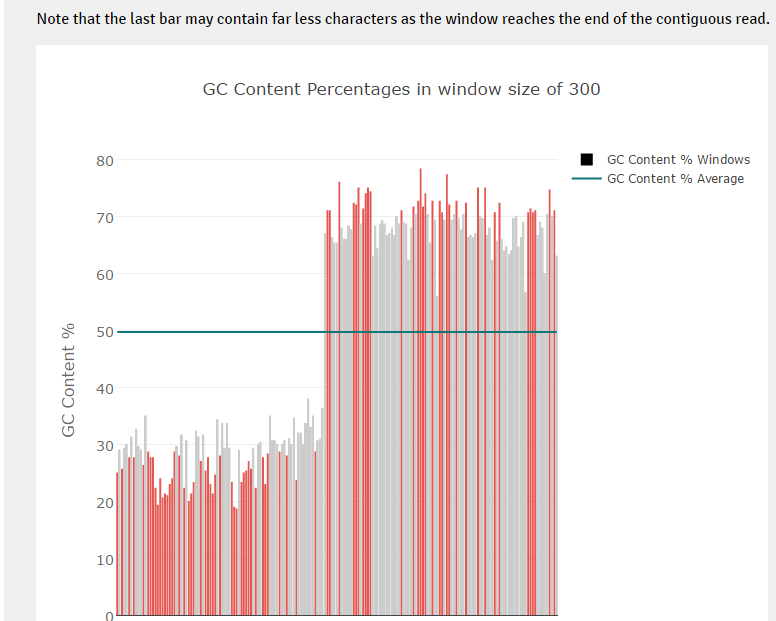
\includegraphics[width=0.7\textwidth]{images/combinedspecies}
\caption{Combining two species contigs together at 50\% of each of the file (first half one species, second half another species), we see a very obvious split in the GC chart.}
\end{figure}

Running this test showed me that it is possible to see where there is a huge change in GC content, but that the threshold won't pick it up because with a case like this, while extremely unlikely to happen where there is a mix of only two species, the threshold only shows those outside of the mean, not drastic changes. It highlights that there is room for improvement with detecting these changes and reporting on them to the user, rather than having them infer it themselves.

\subsubsection{Real Data}
I also tested the application using real metagenomic data. This data was provided by Sam Nicholls, and was taken from the gut of a limpet. There is a large file of thousands of contigs, with the shortest being under a hundred bases long and the longest being above twenty five thousand bases. Running this real data and looking at both the short and long contigs allowed me to see that my application did produce results for displaying areas where there could be chimeric regions in contigs, displaying ORFs and highlighting areas where an ORF may align with a highlighted GC content window.

\subsubsection{Test Table}
For confirming functional requirements were met and testing things that couldn't be done with automation, I produced a test table with tests matching requirements, expected results and avoiding unwanted results. The tests from the table were carried out by fulfilling the action in the table, and then viewing the results and marking whether the expectations were met or not. You can see the System Test Table included in the Appendices.

When it came to running large files, or files with many contigs, I ran a number of my laptop and for the most part it handled them quite well with a few hundred contigs of moderate length, although with contigs in the sizes of a hundred thousand characters and up, the process of reading in the contigs and then processing one starts taking noticeably longer. I believe this is a restriction with my own machine, however, as should the JVM be allotted enough memory while the application is hosted on a larger, faster machine it is likely it could perform far better.

\chapter{Evaluation}

\section{Requirements Analysis}
How well did I assess the requirements of the project? How did this tie into my Project objectives? Did it impact my design? What about selecting to do GC content over k-mer frequency analysis? Paralysis of choice?

\section{Technical Achievement}
Do I think I did something technical? What did I actually learn? Was it useful to learn? Could i have done something better? Did the software meet the requirements set out? was it of good quality? Could the design have been done differently, or is it good? What about my technology decisions?

\subsection{Future Work}
If I were to continue developing this project, what would I begin with, and how would I go from there? 
\subsubsection{Improvements}
What is in the code currently that could be improved? Refactoring? Functionality? Validation
Improvements on the Superframe? Displaying GC content could be done with my own chart rather than with Plotly. Better way of reporting on when GC Content is drastically different. Window sizes that change and slide.
\subsubsection{Additional Functionality}
What do I feel I would like to implement? k-mer frequency analysis? Tie in to BLAST? File submission? More tests on larger systems? Floor is open from there to find other ways of determining quality.

\section{Project Management}
What was my process like? Did I find it helped or hindered? Could I have tried something different or been better at it? What was good about it?

\section{Final Conclusion}
Overall, how do I think the project did?
If I did start the project again, what would I do different (technical, process, etc? )
Did I learn things, domain and technical?

% Examiners expect to find in your dissertation a section addressing such questions as:

%\begin{itemize}
%   \item Were the requirements correctly identified? 
%   \item Were the design decisions correct?
%   \item Could a more suitable set of tools have been chosen?
%   \item How well did the software meet the needs of those who were expecting to use it?
%   \item How well were any other project aims achieved?
%   \item If you were starting again, what would you do differently?
%\end{itemize}

% Such material is regarded as an important part of the dissertation; it should demonstrate that you are capable not only of carrying out a piece of work but also of thinking critically about how you did it and how you might have done it better. This is seen as an important part of an honours degree. 

% There will be good things and room for improvement with any project. As you write this section, identify and discuss the parts of the work that went well and also consider ways in which the work could be improved. 

% Review the discussion on the Evaluation section from the lectures. A recording is available on Blackboard. 

% add any additional chapters here

\setemptyheader
\addcontentsline{toc}{chapter}{Appendices}
\chapter*{Appendices}
\pagebreak

% start the appendix - sets up different numbering
\fancypagestyle{plain}{%
%\fancyhf{} % clear all header and footer fields
\fancyhead[L]{\textsl{Appendix\ \thechapter}}
\fancyhead[R]{\textsl{\leftmark}}}

\appendix
\fancyhead[L]{\textsl{Appendix\ \thechapter}}
\fancyhead[R]{\textsl{\leftmark}}
\fancyhead[C]{}
\fancyfoot[C]{\thepage}
\renewcommand{\headrulewidth}{0.4pt}
\renewcommand{\chaptermark}[1]{\markboth{#1}{}}

\fancyhead[L]{\textsl{Appendix\ \thechapter}}
\fancyhead[R]{\textsl{\leftmark}}
\fancyfoot[C]{{\thepage} of \pageref{LastPage}}

% include any appendices here
\chapter{Third-Party Code and Libraries}

If you have made use of any third party code or software libraries, i.e. any code that you have not designed and written yourself, then you must include this appendix. 

As has been said in lectures, it is acceptable and likely that you will make use of third-party code and software libraries. The key requirement is that we understand what is your original work and what work is based on that of other people. 

Therefore, you need to clearly state what you have used and where the original material can be found. Also, if you have made any changes to the original versions, you must explain what you have changed. 

As an example, you might include a definition such as: 

Apache POI library � The project has been used to read and write Microsoft Excel files (XLS) as part of the interaction with the client�s existing system for processing data. Version 3.10-FINAL was used. The library is open source and it is available from the Apache Software Foundation 
\cite{apache_poi}. The library is released using the Apache License 
\cite{apache_license}. This library was used without modification. 

\chapter{Ethics Submission}

Ethics Application Number: 4295
\newline
Ethics Submission document overleaf.

\includepdf[pages={1,2}]{appendix2/ethicssubmission.pdf}
\chapter{Examples and Extras}

\section{Example User Story Breakdown}
NOTE: This break down is from my blog entry at \url{http://users.aber.ac.uk/jee22/wordpress/?p=147}.
\begin{verbatim}
“As a researcher
I want to get a report on the quality of my metagenome
So that I know whether it is of good or bad quality”
\end{verbatim}
Okay, super high level. This can be broken down into:
\begin{verbatim}
“As a researcher
I want to get a report on the GC content of my metagenome
So that I can see where there might be inconsistencies”
\end{verbatim}
So, that could be explained better (i.e. what are ‘inconsistencies’? Areas where there might be a split/chimera, or just gene encoding regions and completely natural).
\begin{verbatim}
“As a researcher
I want descriptions of the GC content of my metagenome
So that I can pinpoint areas of interest”
\end{verbatim}
Perhaps a better way of making a story for GC content in this instance.
What about the report?
\begin{verbatim}
“As a researcher
I want a textual and graphical description of my metagenome quality
So that I can see and understand where there might be quality issues”
\end{verbatim}
Again, quite high level, but not too bad. This could be broken down further.
\begin{verbatim}
“As a researcher
I want a graph plotted to show me the GC content in my metagenome
So I can visualise the distribution of GC content to better understand my metagenome assembly”
\end{verbatim}
From some of these, further tasks can be broken down, so, lets take one and do that with the last story I defined. I suppose, before we can do that though, since we don’t have an application developed, we might need some initial ‘setup’ stories.
\begin{verbatim}
“As a researcher
I want an application to read in my metagenome assembly
So I can see it outside of the FASTA file”
\end{verbatim}
Maybe that’s pushing it a little. There’s not really much to be gained from this in business value, but, as far as development goes it can give us some nice little tasks:
\begin{verbatim}
Read in FASTA file
Output display of metagenome visually for researcher to understand
\end{verbatim}
That’s just two simple tasks. Read in a file type, and with the contents, display it. It might not be much, but it’s a start where we can say to a hypothetical researcher “Okay, we’ve taken your file, and we can show you that your metagenome looks like this. There’s no processing done to it, but you can see how with this visualisation, there’s the room for labelling and noting the interesting points later. What do you think?”

This story with others could then help us propose a Sprint Goal, as below:

Sprint Goal:
To display a metagenome in an application after reading in a FASTA file, with the look at implementing GC Content counting should time allow.

\section{Artificial Test File}
\begin{verbatim}
>TEST_High_GC_Content_Out_of_frame_mid_difference
CCCGGGCCCGGGCCCGGGCCCGGGCCCGGGCCCGGGCCCGGGCCCGGGCCCGGGCCCGGG
CCCGGGCCCGGGCCCGGGCCCGGGCCCGGGCCCGGGCCCGGGCCCGGGCCCGGGCCCGGG
CCCGGGCCCGGGCCCGGGCCCGGGCCCGGGCCCGGGCCCGGGCCCGGGCCCGGGCCCGGG
CCCGGGCCCGGGCCCGGGCCCGGGCCCGGGCCCGGGCCCGGGCCCGGGCCCGGGCCCGGG
CCCGGGCCCGGGCCCGGGCCCGGGCCCGGGCCCGGGCCCGGGCCCGGGCCCGGGCCCGGG
CCCGGGCCCGGGCCCGGGCCCGGGCCCGGGCCCGGGCCCGGGCCCGGGCCCGGGCCCGGG
CCCGGGCCCGGGCCCGGGCCCGGGCCCGGGCCCGGGCCCGGGCCCGGGCCCGGGCCCGGG
CCCGGGCCCGGGCCCGGGCCCGGGCCCGGGCCCGGGCCCGGGCCCGGGCCCGGGCCCGGG
CCCGGGCCCGGGCCCGGGCCCGGGCCCGGGCCCGGGCCCGGGCCCGGGCCCGGGCCCGGG
CCCGGGCCCGGGCCCGGGCCCGGGCCCGGGCCCGGGCCCGGGCCCGGGCCCGGGCCCGGG
CCCGGGCCCGGGCCCGGGCCCGGGCCCGGGCCCGGGCCCGGGCCCGGGCCCGGGCCCGGG
CCCGGGCCCGGGCCCGGGCCCGGGCCCGGGCCCGGGCCCGGGCCCGGGCCCGGGCCCGGG
CCCGGGCCCGGGCCCGGGCCCGGGCCCGGGCCCGGGCCCGGGCCCGGGCCCGGGCCCGGG
CCCGGGCCCGGGCCCGGGCCCGGGCCCGGGCCCGGGCCCGGGCCCGGGCCCGGGCCCGGG
CCCGGGCCCGGGCCCGGGCCCGGGCCCGGGCCCGGGCCCGGGCCCGGGCCCGGGCCCGGG
CCCGGGCCCGGGCCCGGGCCCGGGCCCGGGCCCGGGCCCGGGCCCGGGCCCGGGCCCGGG
CCCGGGCCCGGGCCCGGGCCCGGGCCCGGGCCCGGGCCCGGGCCCGGGCCCGGGCCCGGG
CCCGGGCCCGGGCCCGGGCCCGGGCCCGGGCCCGGGCCCGGGCCCGGGCCCGGGCCCGGG
ATTATTATTATTATTATTATTATTATTATTATTATTATTATTATTATTATTATTATTATT
ATTATTATTATTATTATTATTATTATTATTATTATTATTATTATTATTATTATTATTATT
ATTATTATTATTATTATTATTATTATTATTATTATTATTATTATTATTATTATTATTATT
ATTATTATTATTATTATTATTATTATTATTATTATTATTATTATTATTATTATTATTATT
CCCGGGCCCGGGCCCGGGCCCGGGCCCGGGCCCGGGCCCGGGCCCGGGCCCGGGCCCGGG
CCCGGGCCCGGGCCCGGGCCCGGGCCCGGGCCCGGGCCCGGGCCCGGGCCCGGGCCCGGG
CCCGGGCCCGGGCCCGGGCCCGGGCCCGGGCCCGGGCCCGGGCCCGGGCCCGGGCCCGGG
CCCGGGCCCGGGCCCGGGCCCGGGCCCGGGCCCGGGCCCGGGCCCGGGCCCGGGCCCGGG
CCCGGGCCCGGGCCCGGGCCCGGGCCCGGGCCCGGGCCCGGGCCCGGGCCCGGGCCCGGG
CCCGGGCCCGGGCCCGGGCCCGGGCCCGGGCCCGGGCCCGGGCCCGGGCCCGGGCCCGGG
CCCGGGCCCGGGCCCGGGCCCGGGCCCGGGCCCGGGCCCGGGCCCGGGCCCGGGCCCGGG
CCCGGGCCCGGGCCCGGGCCCGGGCCCGGGCCCGGGCCCGGGCCCGGGCCCGGGCCCGGG
CCCGGGCCCGGGCCCGGGCCCGGGCCCGGGCCCGGGCCCGGGCCCGGGCCCGGGCCCGGG
CCCGGGCCCGGGCCCGGGCCCGGGCCCGGGCCCGGGCCCGGGCCCGGGCCCGGGCCCGGG
CCCGGGCCCGGGCCCGGGCCCGGGCCCGGGCCCGGGCCCGGGCCCGGGCCCGGGCCCGGG
CCCGGGCCCGGGCCCGGGCCCGGGCCCGGGCCCGGGCCCGGGCCCGGGCCCGGGCCCGGG
CCCGGGCCCGGGCCCGGGCCCGGGCCCGGGCCCGGGCCCGGGCCCGGGCCCGGGCCCGGG
CCCGGGCCCGGGCCCGGGCCCGGGCCCGGGCCCGGGCCCGGGCCCGGGCCCGGGCCCGGG
CCCGGGCCCGGGCCCGGGCCCGGGCCCGGGCCCGGGCCCGGGCCCGGGCCCGGGCCCGGG
CCCGGGCCCGGGCCCGGGCCCGGGCCCGGGCCCGGGCCCGGGCCCGGGCCCGGGCCCGGG
>TEST_Low_GC_Content_In_Frame_Throughout
CCCGGGCCCGGGCCCGGGCCCGGGCCCGGGCCCGGGCCCGGGCCCGGGCCCGGGCCCGGG
CCCGGGCCCGGGCCCGGGCCCGGGCCCGGGCCCGGGCCCGGGCCCGGGCCCGGGCCCGGG
CCCGGGCCCGGGCCCGGGCCCGGGCCCGGGCCCGGGCCCGGGCCCGGGCCCGGGCCCGGG
CCCGGGCCCGGGCCCGGGCCCGGGCCCGGGCCCGGGCCCGGGCCCGGGCCCGGGCCCGGG
CCCGGGCCCGGGCCCGGGCCCGGGCCCGGGCCCGGGCCCGGGCCCGGGCCCGGGCCCGGG
ATGATTATTATTATTATTATTATTATTATTATTATTATTATTATTATTATTATTATTATT
ATTATTATTATTATTATTATTATTATTATTATTATTATTATTATTATTATTATTATTATT
ATTATTATTATTATTATTATTATTATTATTATTATTATTATTATTATTATTATTATTATT
ATTATTATTATTATTATTATTATTATTATTATTATTATTATTATTATTATTATTATTTGA
CCCGGGCCCGGGCCCGGGCCCGGGCCCGGGCCCGGGCCCGGGCCCGGGCCCGGGCCCGGG
CCCGGGCCCGGGCCCGGGCCCGGGCCCGGGCCCGGGCCCGGGCCCGGGCCCGGGCCCGGG
CCCGGGCCCGGGCCCGGGCCCGGGCCCGGGCCCGGGCCCGGGCCCGGGCCCGGGCCCGGG
CCCGGGCCCGGGCCCGGGCCCGGGCCCGGGCCCGGGCCCGGGCCCGGGCCCGGGCCCGGG
>TEST_Sinlge_Frame_Many_Start_Stop_Codons
CCCGGGCCCGGGCCCGGGCCCGGGCCCGGGCCCGGGCCCGGGCCCGGGCCCGGGCCCGGG
ATGGGGCCCGGGCCCGGGCCCGGGCCCGGGCCCGGGCCCGGGCCCGGGCCCGGGCCCGGG
CCCGGGCCCGGGCCCGGGCCCGGGCCCGGGCCCGGGCCCGGGCCCGGGCCCGGGCCCGGG
CCCGGGCCCATGCCCGGGCCCGGGCCCGGGCCCGGGCCCGGGCCCGGGCCCGGGCCCGGG
CCCGGGCCCGGATGCGGGCCCGGGCCCGGGCCCGGGCCCGGGCCCGGGCCCGGGCCCGGG
ATGATTATTATTATTATTATTATTATTATTATTATTATTATTATTATTATTATTATTATT
ATTATTATTATTATTATTATTATTATTATTATTATTATTATTATTATTATTATTATTATT
ATTATTATTATTATTATTATTATTATTATTATTATTATTATTATTATTATTATTATTATT
ATTATTATTATTATTATTATTATTATTATTATTATTATTATTATTATTATTATTATTTGA
CCCGGGCCCGGGCCCGGGCCCGGGCCCGGGCCCGGGCCCGGGCCCGGGCCCGGGCCCGGG
CCCGGGCCCGGGCCCGGGCCCGGGCCCGGGCCCGGGCCCGGGCCTAGGCCCGGGCCCGGG
CCCGGGCCCGGGCCCGGGCCCGGGCCCGGGTAAGGGCCCGGGCCCGGGCCCGGGTGAGGG
CCCGGGCCCGGGCCCGGGCCCGGGCCCGGGCCCGGGCCCGGGCCCGGGCCCGGGCCCGGG
>TEST_50_percent_N_characters
NNNNNNNNNNNNNNNNNNNNNNNNNNNNNNNNNNNNNNNNNNNNNNNNNNNNNNNNNNNN
NNNNNNNNNNNNNNNNNNNNNNNNNNNNNNNNNNNNNNNNNNNNNNNNNNNNNNNNNNNN
NNNNNNNNNNNNNNNNNNNNNNNNNNNNNNNNNNNNNNNNNNNNNNNNNNNNNNNNNNNN
NNNNNNNNNNNNNNNNNNNNNNNNNNNNNNNNNNNNNNNNNNNNNNNNNNNNNNNNNNNN
TTTGGGCCCAAATTTGGGCCCAAATTTGGGCCCAAATTTGGGCCCAAATTTGGGCCCAAA
TTTGGGCCCAAATTTGGGCCCAAATTTGGGCCCAAATTTGGGCCCAAATTTGGGCCCAAA
TTTGGGCCCAAATTTGGGCCCAAATTTGGGCCCAAATTTGGGCCCAAATTTGGGCCCAAA
TTTGGGCCCAAATTTGGGCCCAAATTTGGGCCCAAATTTGGGCCCAAATTTGGGCCCAAA
\end{verbatim}

\fancypagestyle{plain}{%
   \fancyhead{} %[C]{Annotated Bibliography}
   \fancyfoot[C]{{\thepage} of \pageref{LastPage}} % except the center
   \renewcommand{\headrulewidth}{0pt}
   \renewcommand{\footrulewidth}{0pt}
}

\setemptyheader

\nocite{*} % include everything from the bibliography, irrespective of whether it has been referenced.

% the following line is included so that the bibliography is also shown in the table of contents. There is the possibility that this is added to the previous page for the bibliography. To address this, a newline is added so that it appears on the first page for the bibliography. 
\addcontentsline{toc}{chapter}{Annotated Bibliography} % Adds References to contents page

%
% example of including an annotated bibliography. The current style is an author date one. If you want to change, comment out the line and uncomment the subsequent line. You should also modify the packages included at the top (see the notes earlier in the file) and then trash your aux files and re-run. 
%\bibliographystyle{authordate2annot}
\bibliographystyle{IEEEannot}
\renewcommand{\bibname}{Annotated Bibliography} 
\bibliography{References/references} % References file


\end{document}
